%!TEX root = ../thesis.tex

\chapter{BEM with inexact GMRES for the Stokes equation}\label{chapter:stokes}
\thispagestyle{myheadings}

\graphicspath{{Stokes/}}

Now that we have demonstrated the ability of relaxed {\gmres} to correctly solve {\fmmbem} problems based on Laplace's equation and shown the speedups that this approach can give, we can continue to more substantial problems. Results from \S\ref{sec:laplace_relaxation} suggest that as $p$ increases the potential speedup from relaxation also increases. This implies that the benefits from relaxed solvers will increase with a corresponding need for accuracy. The next conclusion we can draw from the Laplace equation tests, is that we can correlate speedups with the number of iterations needed to solve -- in {\gmres} solvers, we spend a majority of iterations with residual values close to the desired final tolerance. As the linear system increases in difficulty to solve, we have more low-precision iterations and it is these iterations that will give us the greatest speedup.

The Stokes equation is a vector equation, and significantly more involved than Laplace, involving $62K$ operations for each $K$-th order integration between two panels, compared to $8K$ for Laplace. It is used in applications such as biomedicine \cite{RahimianETal2010} and MEMS (Microelectromechanical systems)\cite{fachinotti2007}. The use of {\fmmbem} for this equation is also well established \cite{Liu2009,gomez1997}. The difficulty of the resulting problems comes from both the added complications from the equation itself, requiring solving for 3 components (of velocity or surface traction) at every target panel, along with the more difficult linear systems that arise. Additional to these sources of complications, high precision is required in order to maintain accuracy \cite{Liu2009}. This combination of tough linear system, high accuracy and added difficulties within the integrals that must be computed, means we anticipate significant speedups from relaxing the solve, at least on par with those experienced in our Laplace experiments.

\section{Equation}

We start from the unsteady Navier-Stokes equations for fluid motion in terms of the velocity, $\vect{u}$, pressure, $p$, viscocity $\mu$ and fluid density $\rho$,
\begin{equation}
	\label{eqn:navier_stokes}
	\rho\left ( \partiald{\vect{u}}{t} + \vect{u}\cdot\nabla\vect{u}\right ) = -\nabla p + \mu\nabla^{2}\vect{u},
\end{equation}

\noindent
and concentrate on the case where the Reynolds number, $Re_L = \rho UL / \mu$ is small, or in other words,  diffusion effects $\nabla^{2}\vect{u}$ are much larger than convective effects, $\vect{u}\cdot\nabla\vect{u}$.
\begin{equation}
	\nabla^{2}\vect{u} \gg \vect{u}\cdot\nabla\vect{u}
\end{equation}

In this case, we obtain 2 equations, the Stokes equation \eqref{eqn:stokes} and the linearized Navier-Stokes equation \ref{eqn:linearized_ns} for the steady and unsteady cases respectively.
\begin{eqnarray}
	\label{eqn:stokes}\mu\nabla^{2}\vect{u} & = & \nabla p \\
	\label{eqn:linearized_ns}\rho\partiald{\vect{u}}{t} & = & -\nabla p + \mu\nabla^{2}\vect{u}.
\end{eqnarray}

Similar to the Laplace equation, we want the fundamental solution(s) for equation \ref{eqn:stokes}, and these are the Stokeslet \ref{eqn:stokeslet} and the stresslet \ref{eqn:stresslet}, shown in both matrix and tensor notation forms.

%We find that the fundamental solutions to \ref{eqn:stokes} are the stokeslet \ref{eqn:stokeslet}, [[[MORE HERE]]] \ref{eqn:stokeslet_2} 

\begin{eqnarray}
	\label{eqn:stokeslet}
	S_{ij}(\vect{x},\vect{y}) & = & \frac{\delta_{ij}}{r} + \frac{(x_i-y_i)(x_j-y_j)}{r^{3}} \\
	& & \nonumber \\
	\label{eqn:stokeslet_2}
		   & = & \frac{1}{r^{3}}\left (
	\begin{array}{ccc}
		r^{2} + dx^{2} & dx\cdot dy & dx\cdot dz \\
		dx\cdot dy & r^{2} + dy^{2} & dy\cdot dz \\
		dx\cdot dz & dy\cdot dz & r^{2} + dz^{2}
	\end{array} \right )
\end{eqnarray}

%\noindent	
%and the stresslet \ref{eqn:stresslet}, \ref{eqn:stresslet_2}

\begin{eqnarray}
	\label{eqn:stresslet}
	%D_{ij}(\vect{x},\vect{y},\vect{\hat{n}}) & = & \frac{1}{6}\sum_{k=1}^{3}\left [ \left( \delta_{ij} - (x_j-y_j)\partiald{}{x_i}\right ) \frac{(x_k-y_k)\hat{n}_k}{r^{3}} \right . \nonumber \\ 
%& & + \left . \left (\delta_{ik}-(x_k-y_k)\partiald{}{x_i}\right )\frac{(x_j-y_j)\hat{n}_k}{r^{3}}\right ] \\
	T_{ijk}(\vect{x},\vect{y},\nhat) & = & 6\frac{(x_i-y_i)(x_j-y_j)(x_k-y_k)n_k}{r^{5}} \\
	& & \nonumber \\ 
	\label{eqn:stresslet_2}
	& = & 6\frac{(\di{\vect{x}}\cdot\vect{\hat{n}})}{r^{5}}\left (\begin{array}{ccc}
		dx^{2} & dx\cdot dy & dx\cdot dz \\
		dx\cdot dy & dy^{2} & dy\cdot dz \\
		dx\cdot dz & dy\cdot dz & dz^{2}
	\end{array} \right )
\end{eqnarray}

These fundamental solutions will be used in the next section when we formulate a {\bem} form of the Stokes equation, suitable for solving with the framework used throughout this thesis.  
		
\section{BEM}

Similar to how we began from Green's second identity while deriving the boundary integral form of the Laplace equation, we start here from Lorentz's reciprocal relation, similar to standard derivations \cite{Pozrikidis1992,Liu2009}.

\begin{eqnarray}
	\label{eqn:stokes_bem_1}\nabla\cdot\left ( \vect{u}'\cdot\vect{\sigma} - \vect{u}\cdot\vect{\sigma}'\right ) & = & 0 \\
	\label{eqn:stokes_bem_2}\partiald{}{x_k}\left ( u_i'\sigma_{ik} - u_i\sigma_{ik}' \right ) & = & 0,
\end{eqnarray}

\noindent
where $\vect{u}$ and $\vect{u}'$ are solutions to Stokes equations, and $\vect{\sigma}$ and $\vect{\sigma}'$ are the associated stress tensors. Looking at the domain in figure \ref{fig:stokes_volume}, if we identify $\vect{u}'$ as the velocity induced from a point source with strength $\vect{g}$, we can obtain

\begin{figure}[h]
\begin{center}
	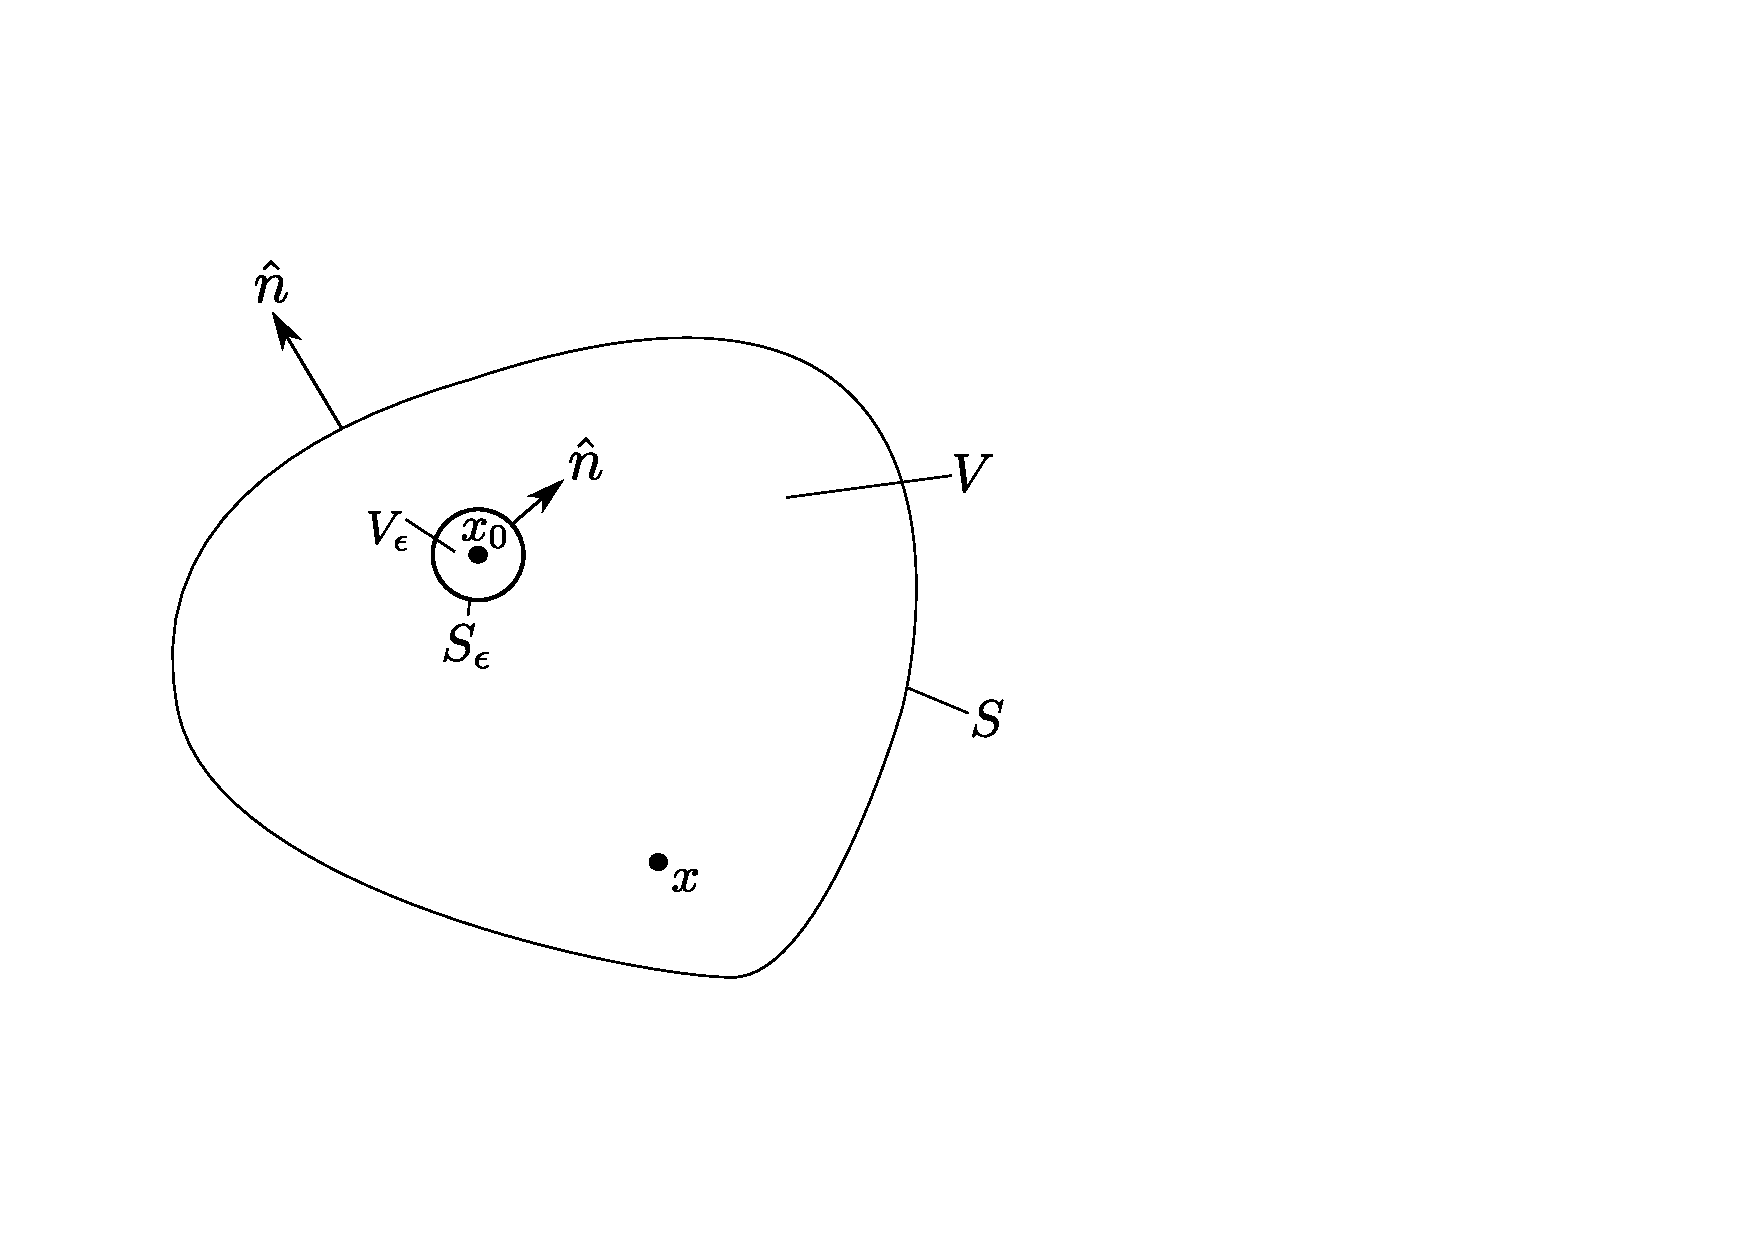
\includegraphics[width=12cm]{img/StokesVolume.pdf}
	\caption{Domain used for derivation of Stokes boundary integral equation}
	\label{fig:stokes_volume}
\end{center}
\end{figure}

\begin{equation}
	\label{eqn:stokes_bem_3} u_i(\vect{x}) = \frac{1}{8\pi\mu}G_{ij}(\vect{x},\vect{x}_0)g_j,\;\;\;\;\sigma_{ijk}' = \frac{1}{8\pi}T_{ij}(\vect{x},\vect{x}_0,\nhat)g_j.
\end{equation}

Discarding $\vect{g}$ as a constant, and substituting \ref{eqn:stokes_bem_3} into \ref{eqn:stokes_bem_2}, we get

\begin{equation}
	\label{eqn:stokes_bem_4}
	\partiald{}{x_k}\left ( G_{ij}(\vect{x},\vect{x}_0)\sigma_{ik}(\vect{x}) - \mu u_i(\vect{x})T_{ijk}(\vect{x},\vect{x}_0)\right ) = 0.
\end{equation}

Next, we integrate \ref{eqn:stokes_bem_4} over a volume, $V$, set $\vect{x}_0$ outside of $V$ and apply the divergence theorem

\begin{equation}
	\label{eqn:stokes_bem_5}
	\int_{\Gamma} \left [ G_{ij}(\vect{x},\vect{x}_0)\sigma_{ik}(\vect{x}) -\mu u_i(\vect{x})T_{ijk}(\vect{x},\vect{x}_0)\right ]\hat{n}_k(\vect{x})\di{\vect{S}}(\vect{x}) = 0.
\end{equation}

Next, moving $\vect{x}_0$ towards the surface, we select $V_\epsilon$ as a small spherical volume around $\vect{x}_0$ with radius $\epsilon$. Integrating over $V-V_\epsilon$ and using the divergence theorem once more

\begin{equation}
	\label{eqn:stokes_bem_6}
	\int_{\Gamma,S_\epsilon} \left [ G_ij(\vect{x},\vect{x}_0)\sigma_{ik}(\vect{x}) -\mu u_i(\vect{x})T_{ijk}(\vect{x},\vect{x}_0)\right ]\hat{n}_k(\vect{x})\di{\vect{S}}(\vect{x}) = 0.
\end{equation}

Letting $\epsilon\to 0$, $\vect{G}, \vect{T}$ reduce to the Stokeslet and stresslet,

\begin{equation}
	\label{eqn:stokes_bem_7}
	G_{ij} = S_{ij} = \frac{\delta_{ij}}{\epsilon} + \frac{\hat{x}_i\hat{x}_j}{\epsilon^{3}}, \;\;\;\; T_{ijk} = -6\frac{\hat{x}_i\hat{x}_j\hat{x}_k}{\epsilon^{5}},
\end{equation}

\noindent
with $\hat{x}_i = x_i - x_{0i}$. Over the volume $S_\epsilon$, $\hat{n} = \hat{x}/\epsilon$ and $\di{\vect{S}} = \epsilon^{2}\di{\Omega}$. Substituting \ref{eqn:stokes_bem_7} into \ref{eqn:stokes_bem_6} we now obtain
\begin{equation}
	\label{eqn:stokes_bem_8}
	\begin{multlined}
	\int_{\Gamma,S_\epsilon} \left [ G_ij(\vect{x},\vect{x}_0)\sigma_{ik}(\vect{x}) -\mu u_i(\vect{x})T_{ijk}(\vect{x},\vect{x}_0)\right ]\hat{n}_k(\vect{x})\di{\vect{S}}(\vect{x}) = \\
	-\int_{S_\epsilon} \left [ \left ( \delta_{ij} + \frac{\hat{x}_i\hat{x}_j}{\epsilon^{2}} \right )\sigma_{ik}(\vect{x}) + 6\mu u_i(\vect{x})\frac{\hat{x}_i\hat{x}_j\hat{x}_k}{\epsilon^{4}} \right ]\hat{x}_k\;\di{\Gamma}.
	\end{multlined}
\end{equation}

When we take the limit $\epsilon\to 0$, $\vect{u}$ and $\vect{\sigma}$ over the volume $S_\epsilon$ tend to $\vect{u}(\vect{x}_0)$ and $\vect{\sigma}(\vect{x}_0)$. We also note that as $\epsilon\to 0$ the stress term on the right-hand-side of \ref{eqn:stokes_bem_8} will decrease linearly, while the velocity term will tend to a constant,

\begin{equation}
	\label{eqn:stokes_bem_9}
	-6\mu u_i(\vect{x}_0)\frac{1}{\epsilon^{4}}\int_{S_\epsilon} \hat{x}_i\hat{x}_j\;\di{S(\vect{x})}.
\end{equation}

Applying the divergence theorem to the surface integral in \ref{eqn:stokes_bem_9}, we get

\begin{equation}
	\label{eqn:stokes_bem_10}
	\int_{S_\epsilon} \hat{x}_i\hat{x}_j\;\di{S(\vect{x})} = \epsilon\int_{S_\epsilon}\hat{x}_i\hat{n}_j\;\di{S(\vect{x})} = \epsilon\int_{V_\epsilon}\partiald{\hat{x}_i}{\hat{x}_j}\;\di{V(\vect{x})} = \delta_{ij}\frac{4}{3}\pi\epsilon^{4}.
\end{equation}

Finally plugging \ref{eqn:stokes_bem_10} into \ref{eqn:stokes_bem_8} (with the right hand side collapsed to \ref{eqn:stokes_bem_9}), we get the expected boundary integral form:

\begin{equation}
	\label{eqn:stokes_bem_11}
	u_j(\vect{x_0}) = -\frac{1}{8\pi\mu}\int_{\Gamma} \sigma_{ik}(\vect{x})n_k(\vect{x})G_{ij}(\vect{x},\vect{x}_0)\;\di{S(\vect{x})} + \frac{1}{8\pi} \int_{\Gamma} u_i(\vect{x})T_{ijk}(\vect{x},\vect{x}_0)n_k(\vect{x})\;\di{S(\vect{x})}.
\end{equation}

Setting $t = \sigma\cdot\nhat$ and taking $\vect{x}_0$ to a smooth part of the boundary, \\
$\int_{\Gamma} u_i(\vect{x})T_{ijk}(\vect{x},\vect{x}_0)n_k(\vect{x})\;\di{\Gamma(\vect{x})} \to 0$, and $\int_{\Gamma} \sigma_{ik}(\vect{x})n_k(\vect{x})G_{ij}(\vect{x},\vect{x}_0)\;\di{\Gamma(\vect{x})} \to 1/2$. This gives the final form of the boundary integral equation before discretization

%Taking $\vect{x}_0$ to the boundary, and setting $t = \sigma\nhat$, we introduce a constant, $c_{ij}$ in front of the initial $u_j$, and when we take $\vect{x}_0$ to the centre of a smooth surface (such as in collocation) $c_{ij} = \delta_{ij}\frac{1}{2}$. Applying this to \ref{eqn:stokes_bem_11} along with denoting the surface traction force, $\vect{t}(\vect{x}) = \sigma_{ik}(\vect{x})n_k(\vect{x})$, we obtain the final, implemented form of the boundary integral equation

\begin{equation}
	\label{eqn:stokes_bem_12}
	\frac{1}{2}u(\vect{x_0}) = -\frac{1}{8\pi\mu}\int_{\Gamma} t_i(\vect{x})G_{ij}(\vect{x},\vect{x}_0)\;\di{\Gamma} + \frac{1}{8\pi} \int_{\Gamma} u_i(\vect{x})T_{ijk}(\vect{x},\vect{x}_0)n_k(\vect{x})\;\di{\Gamma}.
\end{equation}

Finally discretizing with constant panels we obtain

\begin{equation}
	\label{eqn:stokes_bem_discretized}
	\frac{1}{2}u_i(\vect{x_0}) = -\frac{1}{8\pi\mu}\sum_{j=1}^{N}t_j\int_{\Gamma} G_{ij}\;\di{\Gamma_j} + \frac{1}{8\pi} \sum_{j=0}^{N}u_j\int_{\Gamma} T_{ijk}\cdot n_k\;\di{\Gamma_j}.
\end{equation}

\section{Expansions}\label{sec:stokes_expansions}

To approximate the Stokeslet and stresslet we use a method based on decomposing \ref{eqn:stokeslet} and \ref{eqn:stresslet} into sets of harmonic equations, each suitable to be approximated using the Laplace FMM from \S\ref{sec:laplace_expansions} and recombined to give the full answer \cite{tornberg2008}.

First, we can write the Stokeslet $S_{ij}$ as
\begin{equation}
	S_{ij} = \left ( \delta_{ij} - (x_j-y_j)\partiald{}{x_i}\right)\frac{1}{|\vect{x}_i-\vect{x}_j|},
\end{equation}

\noindent
and $F_i^{m} = F_i(\vect{x}_m)$ as
\begin{equation}
	F_i^{m} = \sum_{n=0}^{N} S_{ij}(\vect{x}_m,\vect{x}_n)\cdot \vect{f}_n
\end{equation}

Then, we can perform more manipulations to get another alternate form,

\begin{equation}
	F_i^{m} = \sum_{j=1}^{3}\left [ \left (\delta_{ij}-x_j^{m}\partiald{}{x_i}\right) \sum_{n=1}^{N}\frac{f^{n}_j}{r_{nm}} \right ] + \partiald{}{x_i}\sum_{n=1}^{N}\frac{\vect{x}^{n}\cdot \vect{f}^{n}}{r_{nm}}.
\end{equation}

This decomposition lets us approximate the Green's function operator with 4 Laplace {\fmm}s for $1/r$, with  source strengths $f^{n}_1,\;f^{n}_2,\;f^{n}_3,\;(\vect{x}^{n}\cdot\vect{f}^{n})$. Similarly, we can rewrite the stresslet, $D_{ij}$ in a similar form:

\begin{equation}
	\begin{multlined}
	D_{ij}(\vect{x},\vect{y},\nhat) = \frac{1}{6}\sum_{k=1}^{3} \left [ \left ( \delta_{ij} - (x_j-y_j)\partiald{}{x_i} \right )\frac{(x_k-y_k)\nhat_k}{|\vect{x}-\vect{y}|^{3}} \right . \\
	+ \left . \left ( \delta_{ik}-(x_k-y_k)\partiald{}{x_i}\right )\frac{(x_j-y_j)\nhat_k}{|\vect{x}-\vect{y}|^{3}} \right ]
	\end{multlined}
\end{equation}

\noindent
and $G_i^{m} = G_i(\vect{x}_m)$ as

\begin{equation}
	G_i^{m} = \sum_{n=0}^{N} D(\vect{x}_m,\vect{x}_n,\nhat_n)\cdot\vect{g}_n
\end{equation}

\begin{equation}
	\begin{multlined}
	G_i^{m} = \frac{1}{6}\sum_{j=1}^{3} \left [ \left ( \delta_{ij}-x_j^{m}\partiald{}{x_i}\right ) \sum_{n=1}^{N} \left \{ \frac{(\vect{r}_{nm}\cdot\vect{\nhat}^{n})g^{n}_{j}}{r_{nm}^{3}} + \frac{(\vect{r}_{nm}\cdot\vect{g}^{n})\nhat^{n}_{j}}{r_{nm}^{3}} \right \} \right ] \\
	+ \frac{1}{6}\partiald{}{x_i}\sum_{n=1}^{N} \left \{ \frac{(\vect{r}_{nm}\cdot\vect{\nhat}^{n})(\vect{x}^{n}\cdot\vect{g}^{n})}{r_{nm}^{3}} + \frac{ (\vect{r}_{nm}\cdot\vect{g}^{n})(\vect{\nhat}^{n}\cdot\vect{x}^{n})}{r_{nm}^{3}} \right \}
	\end{multlined}
\end{equation}

Similar to the Stokeslet case, we are able to approximate the Stresslet using 4 harmonic approximations, this time for $1/r^{3}$, where every particle contributes 2 dipoles to each approximation. 

\begin{eqnarray}
	& &(\vect{r}_{nm}\cdot\vect{\nhat}^{n})g^{n}_{1} + (\vect{r}_{nm}\cdot\vect{g}^{n})\nhat^{n}_{1} \\
	& &(\vect{r}_{nm}\cdot\vect{\nhat}^{n})g^{n}_{2} + (\vect{r}_{nm}\cdot\vect{g}^{n})\nhat^{n}_{2} \\
	& &(\vect{r}_{nm}\cdot\vect{\nhat}^{n})g^{n}_{3} + (\vect{r}_{nm}\cdot\vect{g}^{n})\nhat^{n}_{3} \\
	& &(\vect{r}_{nm}\cdot\vect{\nhat}^{n})(\vect{x}^{n}\cdot\vect{g}^{n}) + (\vect{r}_{nm}\cdot\vect{g}^{n})(\vect{\nhat}^{n}\cdot\vect{x}^{n})
\end{eqnarray}�
%
%\begin{eqnarray}
%	M_1 & = & \sum_{n=1}^{N} \left \{\frac{(\vect{r}_{nm}\cdot\vect{\nhat}^{n})g^{n}_{1}}{r_{nm}^{3}} + \frac{(\vect{r}_{nm}\cdot\vect{g}^{n})\nhat^{n}_{1}}{r_{nm}^{3}} \right \}\\
%	M_2 & = & \sum_{n=1}^{N}\left\{\frac{(\vect{r}_{nm}\cdot\vect{\nhat}^{n})g^{n}_{2}}{r_{nm}^{3}} + \frac{(\vect{r}_{nm}\cdot\vect{g}^{n})\nhat^{n}_{2}}{r_{nm}^{3}}\right\} \\
%	M_3 & = & \sum_{n=1}^{N}\left\{\frac{(\vect{r}_{nm}\cdot\vect{\nhat}^{n})g^{n}_{3}}{r_{nm}^{3}} + \frac{(\vect{r}_{nm}\cdot\vect{g}^{n})\nhat^{n}_{3}}{r_{nm}^{3}}\right\} \\
%	M_4 & = & \sum_{n=1}^{N}\left\{\frac{(\vect{r}_{nm}\cdot\vect{\nhat}^{n})(\vect{x}^{n}\cdot\vect{g}^{n})}{r_{nm}^{3}} + \frac{ (\vect{r}_{nm}\cdot\vect{g}^{n})(\vect{\nhat}^{n}\cdot\vect{x}^{n})}{r_{nm}^{3}}\right\}
%\end{eqnarray}

When we come to evaluate all of these expansions, we note that both the Stokeslet and stresslet are of the same form, just with different source strengths for each expansions. Assuming our 4 expansions $M_i,\;i=1..4$ are ordered in the same way we defined the influences of particles earlier,

\begin{equation}
	\phi^{m}_i = \sum_{j=1}^{3} \left ( \delta_{ij} - x_j^{m}\partiald{}{x_i}\right ) M_j + \partiald{}{x_i}M_4.
\end{equation}

\section{Convergence}\label{sec:stokes_convergence}

Just as for the Laplace equation, we wish to show our method is working as intended, and thus converges to the correct accuracy as a function of the spatial discretization. For the Stokes equations, we choose to simulate the low-Reynolds number flow over a sphere. A classical problem in Stokes flow, when placed in a uniform flow of speed $u_x$, the drag over the sphere can be found analytically to be $F_d = 6\pi\mu Ru_x$.

Imposing $\vect{u} = (1,0,0)^{T}$ at the center of every panel, we solve a first-kind equation for the traction force, $\vect{t}$, from which we can then get the total drag force from the integral

\begin{equation}
	\label{eqn:stokes_traction_drag}
	F_d = \int_\Gamma t_x\;\di{\Gamma'} = \sum_{j=1}^{N} t_{x_j}\cdot A_j
\end{equation}

In these tests, we set $R=1$, $u_x = 1$ and $\mu = 10^{-3}$, giving a drag force of $F_d = 0.01885$. For each case, $p$ was increased until the solution stopped improving. Figure \ref{fig:stokes_sphere_traction} shows the $t_x$, the traction force exerted in the $x$-direction on the sphere

\begin{figure}[h]
\begin{center}
	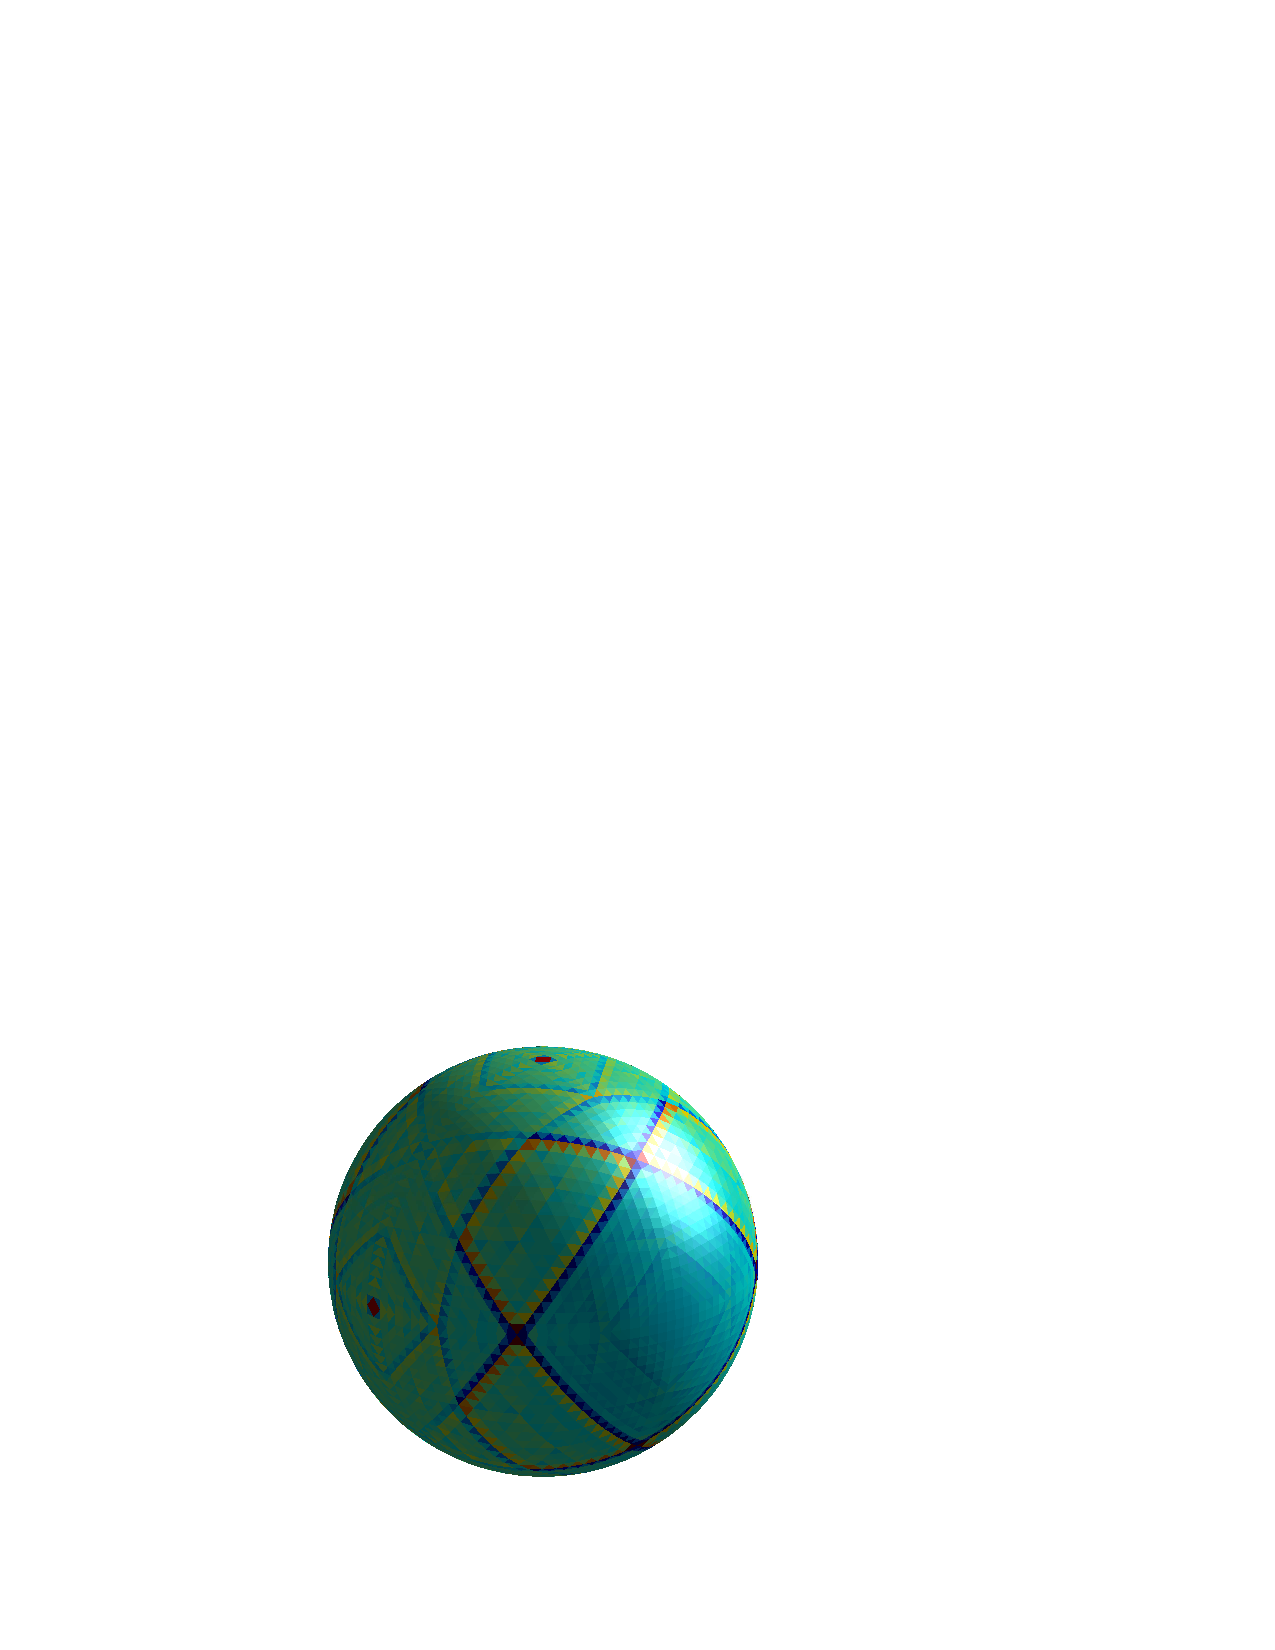
\includegraphics[width=12cm]{img/StokesTraction2.pdf}
	\caption{Traction force $t_x$ exerted in the $x$-direction on a sphere, 32768 panels, $p=16$, $\pmin=5$ solved to $10^{-5}$ tolerance.}
	\label{fig:stokes_sphere_traction}
\end{center}
\end{figure}

It is worth pointing out that while we do have some oscillations in the traction force, their magnitude is small ($\O{10^{-4}}$), and they do not affect the derived quantity (in this case, total drag force) that we are interested in.

\begin{figure}[h]
\begin{center}
	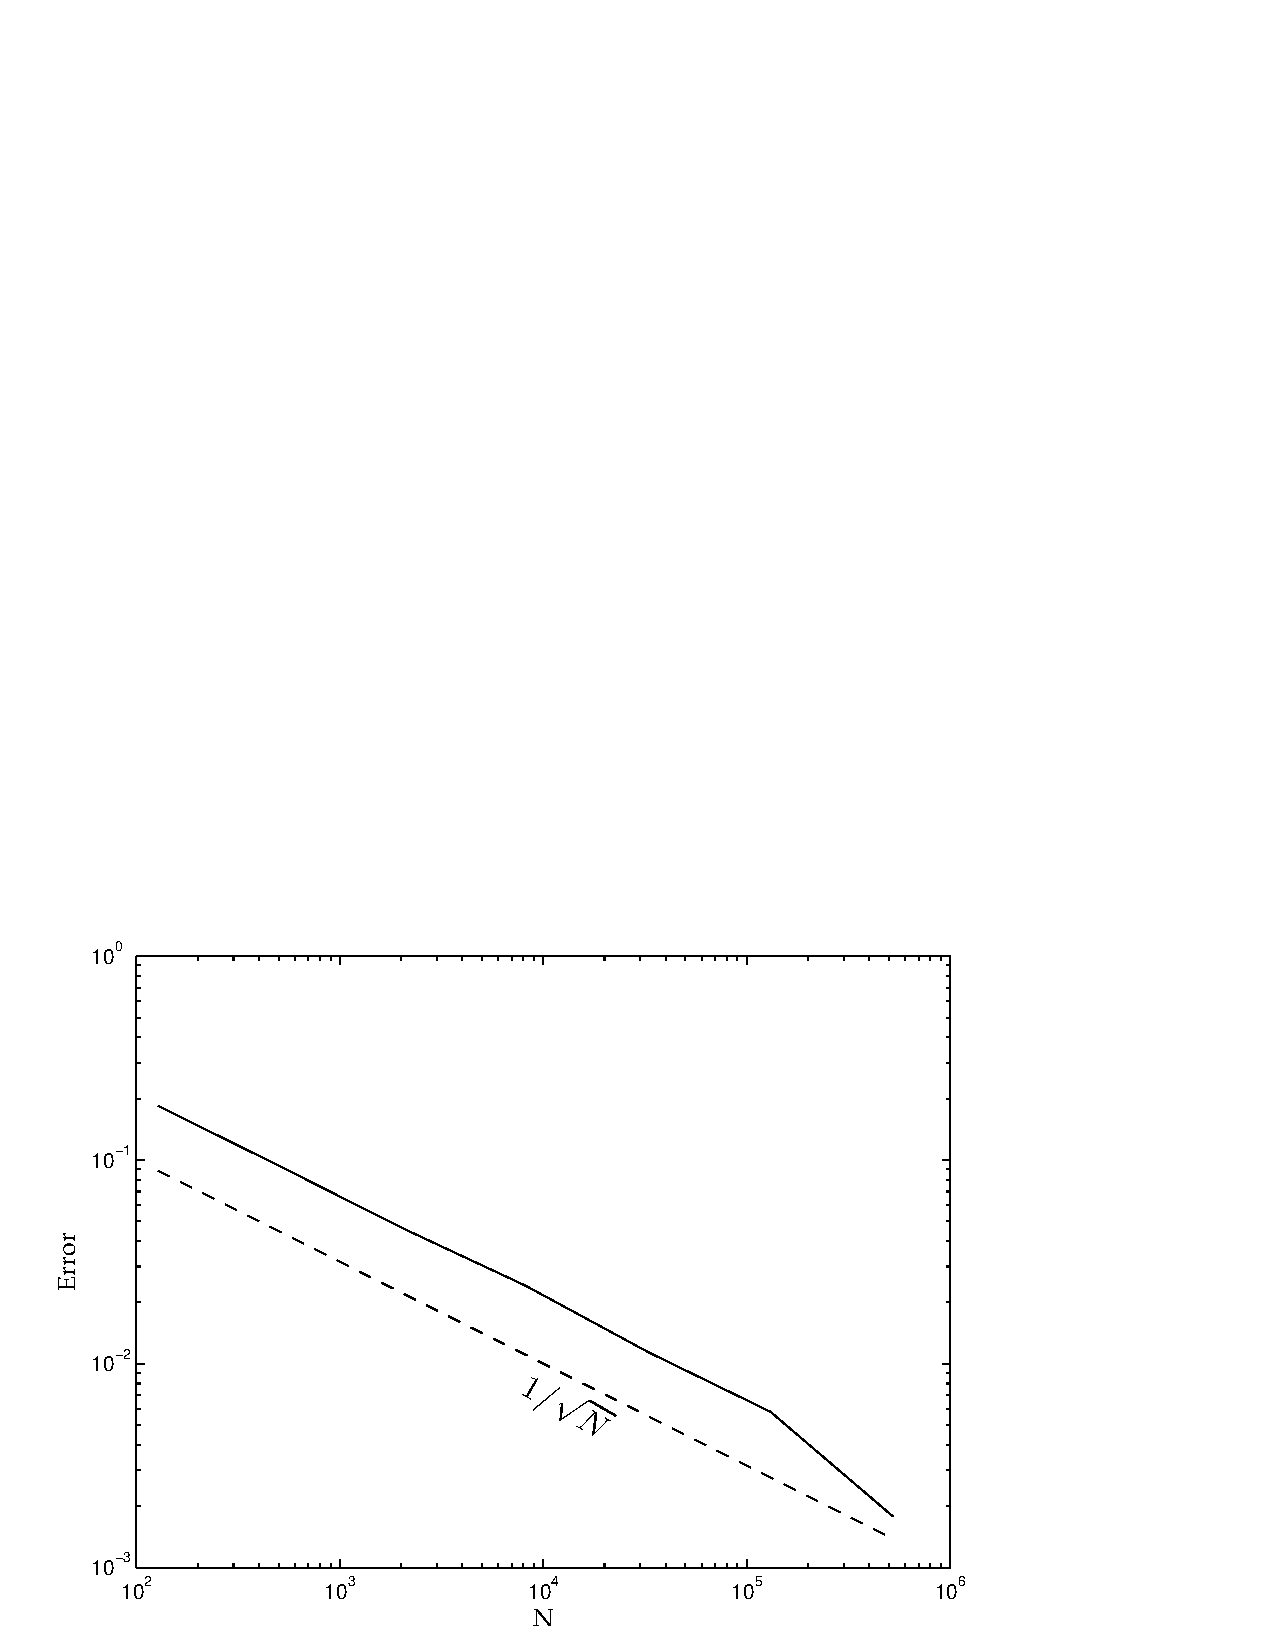
\includegraphics[width=14cm]{img/StokesConvergence.pdf}
	\caption{Convergence of first-kind equation for Stokes flow around a sphere. Initial $p=16$, linear system solved to $10^{-5}$ tolerance.}
	\label{fig:stokes_convergence}
\end{center}
\end{figure}

As shown in figure \ref{fig:stokes_convergence} we see that for 1st-kind equations (likely to be the most common for Stokes problems -- the velocity is prescribed and we wish to find the surface traction), we converge as $\O{1 / \sqrt{N}}$, in-line with the results from \S\ref{sec:laplace_convergence} for the Laplace equation.

%While we would naturally prefer to scale as $\O{1/N}$ or better, this is in-line with the results from \ref{sec:laplace_convergence} for the Laplace equation.

\section{Relaxation}\label{sec:stokes_sphere_relaxation}

Similar to the Laplace equation, we are interested in showing both that using a relaxation scheme converges to the same solution (and thus error) as a non-relaxed run, and that we get a benefit in terms of speed.

First, to estimate the benefits we might obtain, we look at the residual history of a solve for the traction force on a sphere, the same test used in \S\ref{sec:stokes_convergence}. Figure \ref{fig:stokes_residual_history_relaxed} shows that beyond an initial fast reduction in residual in the first 3-4 iterations, before convergence slows until we reach the final residual after $27$ iterations. This is encouraging for the use of relaxation, as we quickly reach a residual that will allow us to dramatically reduce the accuracy needed for the matvec.

It is this reduction in accuracy that we anticipate producing large time savings for the Stokes equations. As the {\fmm} expansions for Stokes consist of $4$ Laplace expansions, and each expansion translation scales as $\O{p^{4}}$, the potential savings are large. For instance, starting a problem with $p=16$ as above, and finishing at $p=5$, the far-field evaluation for each low-accuracy iteration will be approximately $100\times$ faster than the high-precision iteration.

\begin{figure}[h]
\begin{center}
	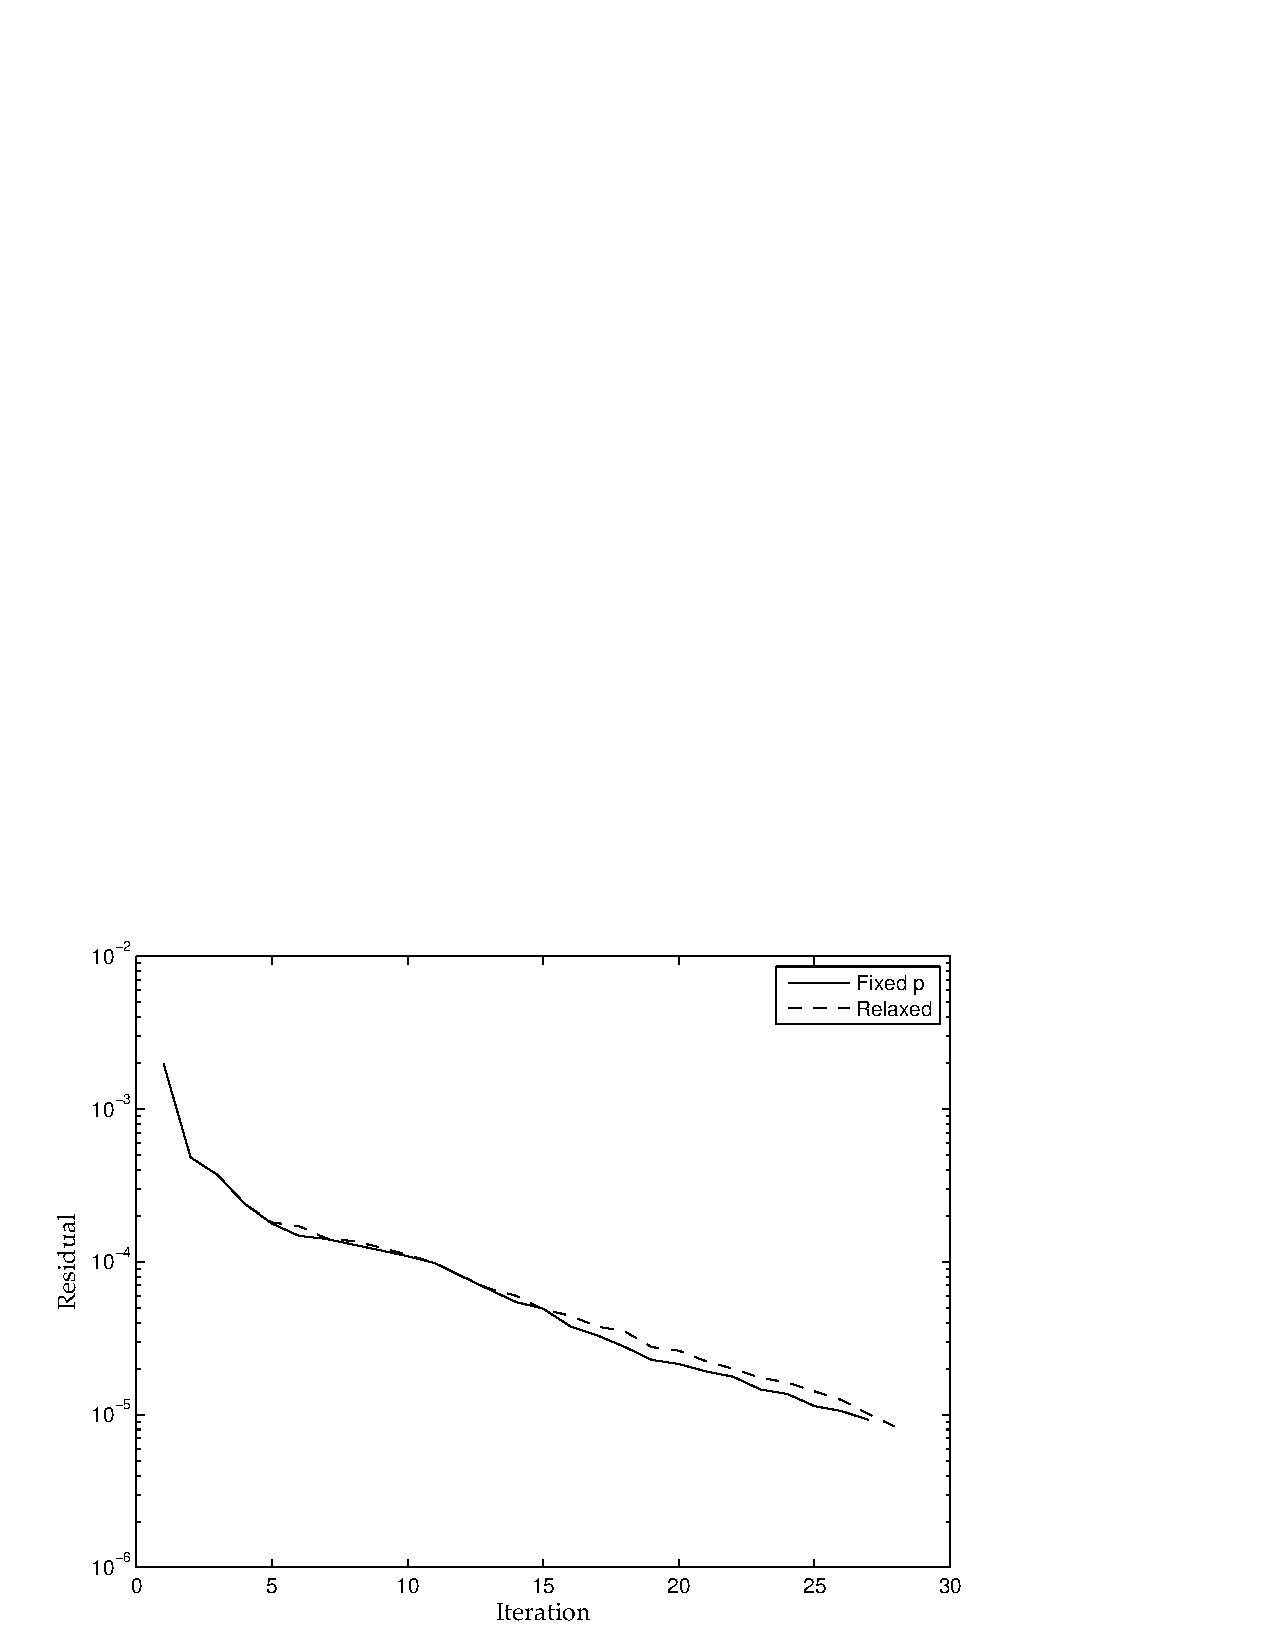
\includegraphics[width=14cm]{img/StokesResidualHistoryRelaxed.pdf}
	\caption{Residual history solving for surface traction on the surface of a sphere, $10^{-5}$ solver tolerance, $8192$ panels, $p=16$.}
	\label{fig:stokes_residual_history_relaxed}
\end{center}
\end{figure}

During this period of initial testing, we confirmed the departure from standard {\fmm} practice as regards to choosing $\ncrit$ and $p$ that we first encountered in \S\ref{sec:laplace_relaxation} for the Laplace equation. Traditionally, we would try to balance the amount of time spent on the near-field ({\ptop}) and far-field (dominated by {\mtol}). While this works well for the case where we keep $p$ constant, it requires an adjustment for the relaxed case. In order for the optimal time to solution, we actually want to balance near and far-fields for the value of $p$ we spend most time on --- in the majority of cases, this is \emph{the lowest instance of $p$}. Figure \ref{fig:stokes_relaxation_breakdown} shows the residual history of a solver over a sphere, along with the breakdown of {\ptop} and {\mtol} for each iteration.

During the verification of our relaxed solver, we encountered a new issue unseen for the Laplace equation in chapter \ref{chapter:laplace_bem}, the need to enforce a \emph{minimum $p$} in order to maintain accuracy. We ran extensive tests on the smallest value of $p$ that could be allowed within the relaxed solver, whilst still maintaining both accuracy and convergence properties. Some of these results are summarized in table \ref{tab:stokes_min_p}.

\begin{table}[htdp]
\begin{center}
\begin{tabular}{c|cc|cc|cc}
  & \multicolumn{2}{c|}{2048 panels} & \multicolumn{2}{c|}{8192 panels} & \multicolumn{2}{c}{32768 panels} \\
 $\pmin$ & Error & $it$ & Error & $it$ & Error & $it$ \\ \hline
  & & & & & & \\
 5 & $4.70\times 10^{-2}$ & 22 & $2.44\times 10^{-2}$ & 28 & $1.34\times 10^{-2}$ & 28 \\
  & & & & & & \\
 4 & $4.49\times 10^{-2}$ & 23 & $2.51\times 10^{-2}$ & 29 & $1.25\times 10^{-2}$ & 29 \\
  & & & & & & \\ 
 3 & $4.64\times 10^{-2}$ & 22 & $2.78\times 10^{-2}$ & 29 & $1.39\times 10^{-2}$ & 29 \\
  & & & & & & \\
 2 & $4.95\times 10^{-2}$ & 25 & $2.62\times 10^{-2}$ & 33 & $3.18\times 10^{-2}$ & 39 \\
  & & & & & & \\
 1 & $4.96\times 10^{-2}$ & 25 & $2.99\times 10^{-2}$ & 51 & $4.77\times 10^{-2}$ & 53 
\end{tabular}
\end{center}
\caption{Effect of $p_{\text{min}}$ on accuracy and convergence for Stokes flow around a sphere for differing values of $N$. Error is on the total drag force in the $x$-direction, $F_x$.}
\label{tab:stokes_min_p}
\end{table}%

These results show that as we discretize more finely, the value of $\pmin$ becomes ever more important. While for 2048 panels, the effect in terms of both accuracy and iteration count is small, it becomes more noticeable at 8192 panels -- with $\pmin = 1$ we require almost twice as many iterations to converge to our tolerance with respect to $\pmin=5$. With 32768 panels, the problems become even more noticeable, with accuracy severely affected at $\pmin=2$ and below. This loss of accuracy is so large that for $\pmin=1$ the error is almost $4\times$ worse than for $\pmin=5$.

Due to this behaviour, we choose to prioritize accuracy over some speed gains and use $\pmin=5$ for all further Stokes flow cases seen in this thesis. We will lose some potential speedups from iterations at even lower values of $p$, but for all cases tried in the course of the experimentation for this thesis, $\pmin=5$ has produced accurate results with good convergence properties.

\begin{figure}[h]
\begin{center}
	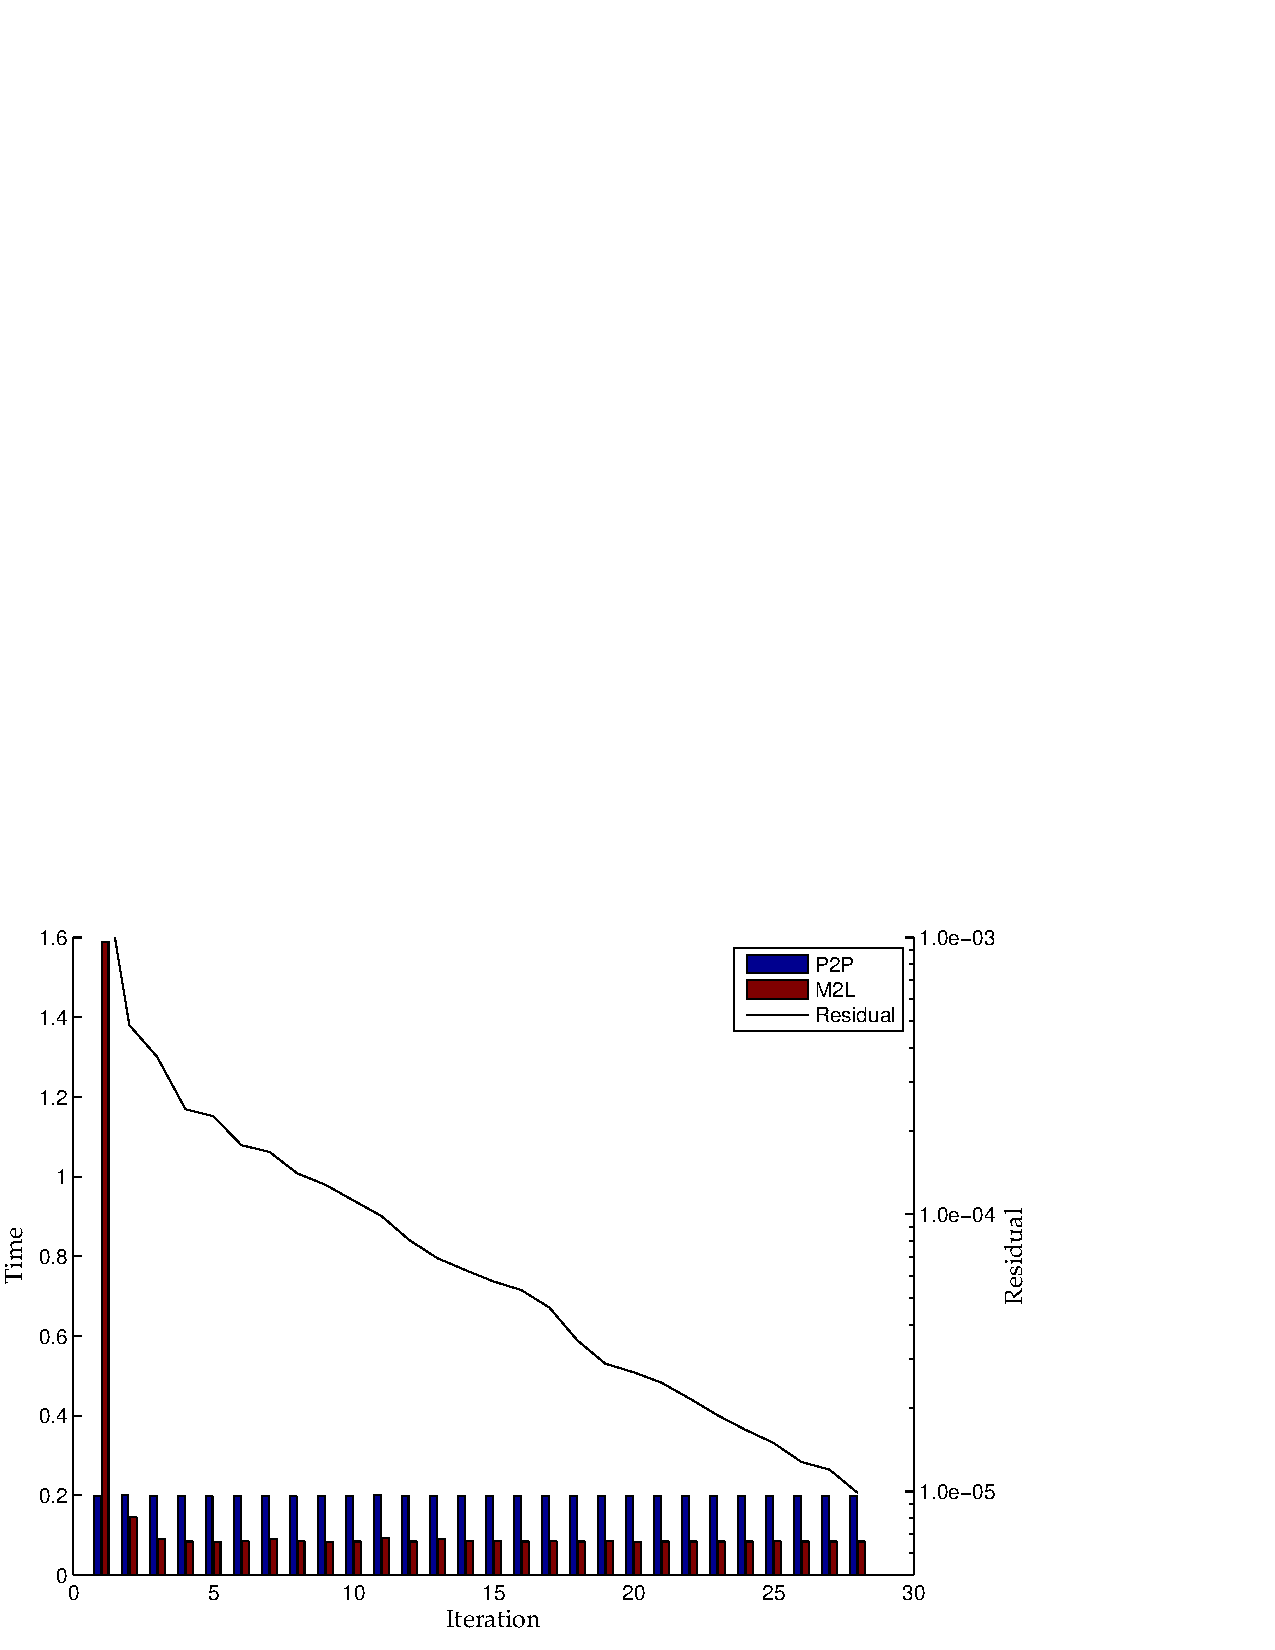
\includegraphics[width=14cm]{img/StokesRelaxationBreakdown.pdf}
	\caption{Residual history solving for surface traction on the surface of a sphere, with time breakdown between {\ptop} and {\mtol}. $10^{-5}$ solver tolerance, $8192$ panels, $p=16$.}
	\label{fig:stokes_relaxation_breakdown}
\end{center}
\end{figure}

The results shown in figure \ref{fig:stokes_relaxation_breakdown} indicate that we spend the vast majority of iterations at the minimum $p$, so, confirming our observation from chapter \ref{chapter:laplace_bem} and the Laplace equation, it is in our best interests to balance the computation for low $p$ case. In practise, this means setting $\ncrit$ to the lowest possible in order to maintain the accuracy of the {\fmm}, as the {\mtol} component becomes very fast at the lowest values of $p$.

After exploring the behavior of the relaxed solver, we can finally present speedup results. Figure \ref{fig:stokes_speedup} shows the speedup of the relaxed solver over keeping $p$ fixed for $N=2048$ to $131072$ (6144 to 393216 unknowns).

\begin{figure}[h]
\begin{center}
	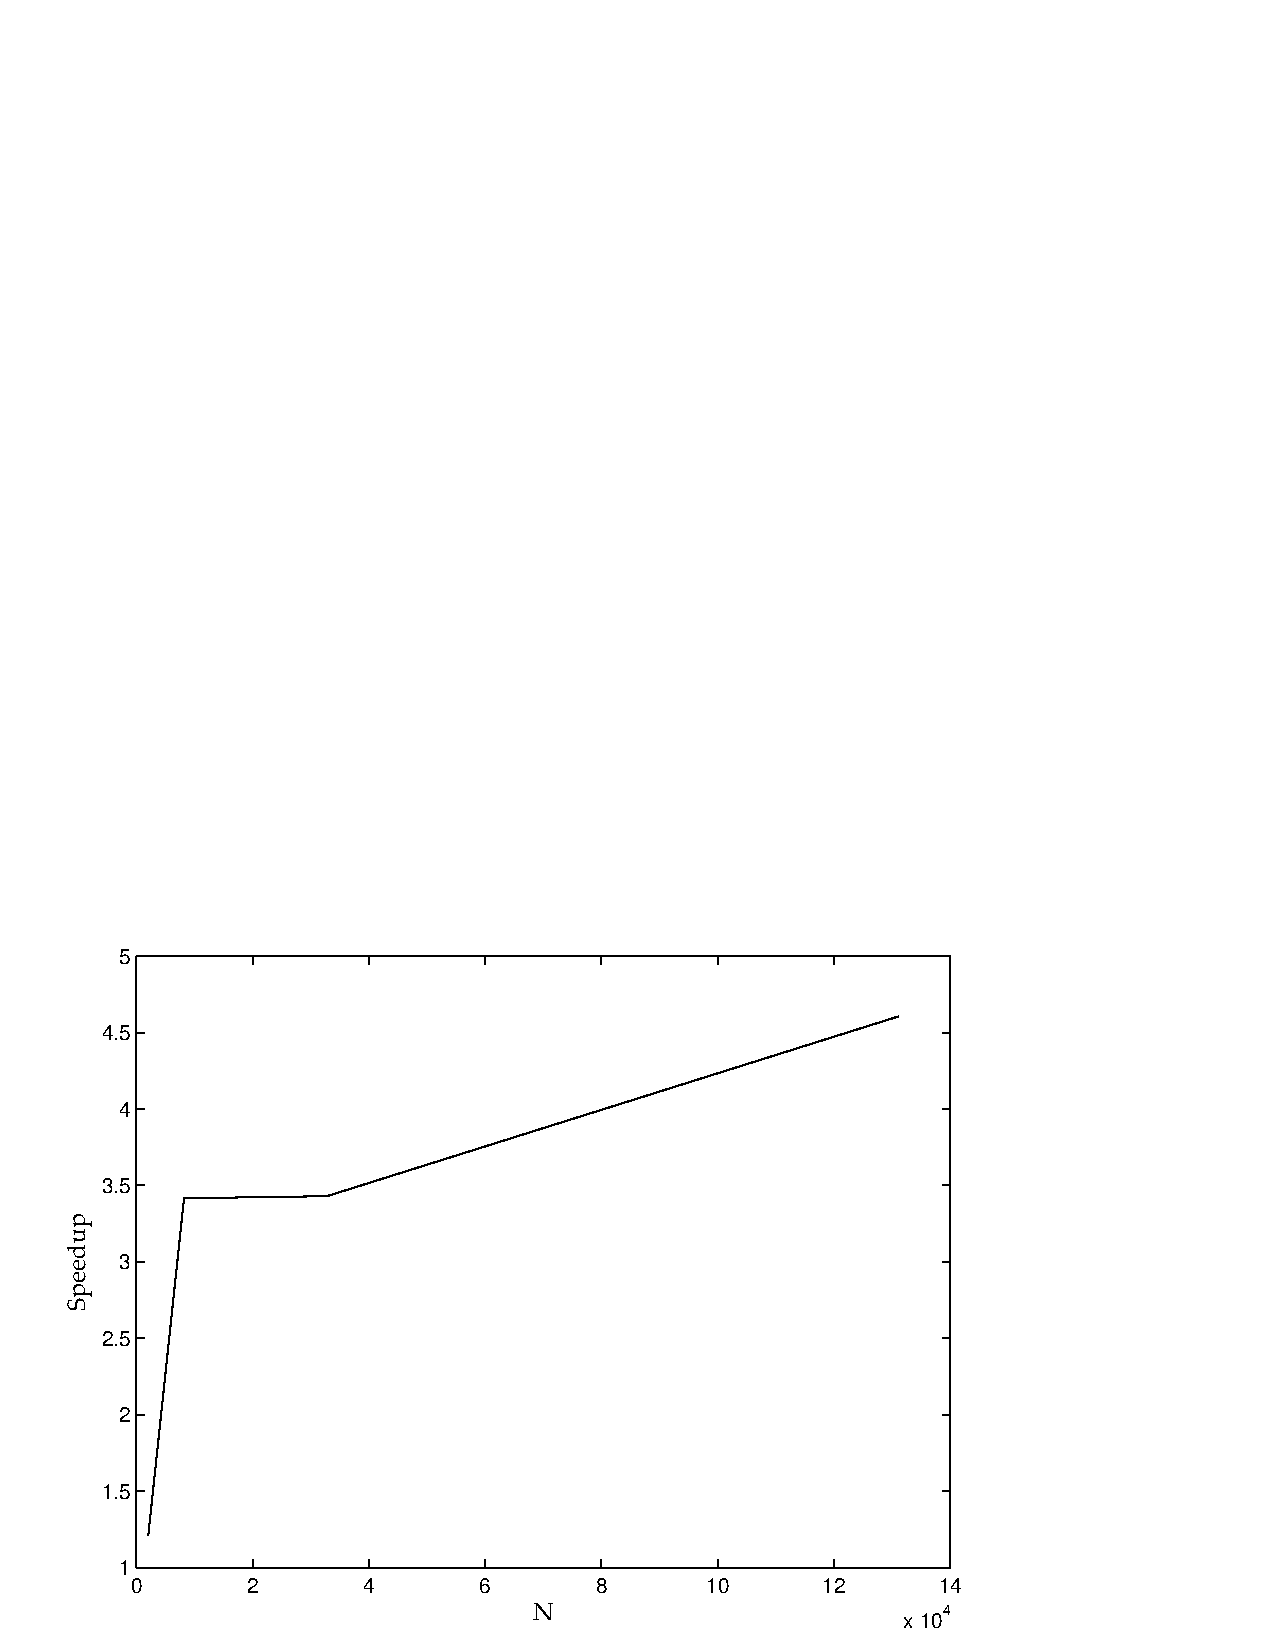
\includegraphics[width=14cm]{img/StokesSpeedup.pdf}
	\caption{Speedup for solving first-kind Stokes equation on the surface of a sphere, varying $N$. $10^{-5}$ solver tolerance, $p=16$. }
	%\caption{Residual history solving for surface traction on the surface of a sphere, with time breakdown between {\ptop} and {\mtol}. $10^{-5}$ solver tolerance, $8192$ panels, $p=16$.}
	\label{fig:stokes_speedup}
\end{center}
\end{figure}

These results demonstrate that our optimism about the potential of relaxed solvers for Stokse problems was clearly warranted. Speedups for problems of $8192$ panels and more are $3.5\times$ or greater, and as problem sizes grow, the speedup increased to greater than $4\times$. This additional speedup for large problems is due to the disparity in $\ncrit$ values needed for relaxed and fixed $p$ cases, and the use of the sparse matrix near-field form from \S\ref{sec:fmm_near_field} -- the higher $\ncrit$ for fixed $p$ problems prohibits the use of the significantly faster sparse matrix approach due to memory consumption.
 
\section{Conclusions}\label{sec:stokes_conclusions}

In this section of the thesis, we have extended the work from chapter \ref{chapter:laplace_bem} to the Stokes equations, a significantly more difficult problem. Our implementation has been shown to converge to the correct solution for a standard test case, and we have demonstrated that as predicted, the combination of high-accuracy and large iteration counts for this type of problem has resulted in good speedups from a relaxed solver, reducing the time-to-solution by a factor of $3-4\times$. Further to these performance results, we have also shown the importance of setting a minimum value of $p$, $\pmin$, that we cannot relax below, in order to maintain accuracy. For all tests performed, $\pmin=5$ was good for minimizing iteration counts while maintaining accuracy. For general problems, the choice of $\pmin$ may be more difficult, requiring either a conservative choice to ensure accuracy, or multiple experiments with varying values of $\pmin$ so that any changes in the solution can be observed.
